\section{Polarization}
\label{sec:polarization}

William Hilter and John Hall first observed polarization of starlight in 1949 \citep{hiltner1949polarization,hall1949observations}.
Polarization was soon linked to magnetic fields of the galaxy 
by Leverrett Davis, Jr. and Jesse Greenstein \citep{davis1951polarization}.

Pulsars have strong magnetic fields which gives rise to not only their 
extremely focused beam of emission but also coherent light with 
defined polarization.  
Polarization is a means of observing the magnetic field lines of these incredibly small,
far away objects.  That we can make such a bold measurement speaks to the extremes of the
pulsar.


Polarization is most often reported in terms of Stokes parameters, $I$, $Q$, $U$, and $V$.
Stokes parameters are a standard way of representing polarization.
At a radio telescope with polarization measurement capabilities, the incoming
electromagnetic wave is converted to electric voltage in two independent
feeds.  Linear feeds will measure polarization aligned along $x$ and $y$ Cartesian coordinates
while circular feeds will measure polarization as right-handed or left-handed.

Components of the linear and circular feeds can be converted to Stokes parameters
\begin{equation}
 \begin{array}{lcl}
    I=\langle E_{\rm X}^{2} \rangle + \langle E_{\rm Y}^{2} \rangle &\textrm{and}& I=\langle E_{\rm R}^{2} \rangle + \langle E_{\rm L}^{2} \rangle,\\
    Q=\langle E_{\rm X}^{2} \rangle - \langle E_{\rm Y}^{2} \rangle &\textrm{and}& Q=2\langle E_{\rm R}^{2} E_{\rm L}^{2} \cos {\left(\kappa_{\rm RL}\right)} \rangle,\\
    U=2\langle E_{\rm R}^{2} E_{\rm L}^{2} \cos {\left(\kappa_{\rm XY}\right)} \rangle &\textrm{and}& U=2\langle E_{\rm R}^{2} E_{\rm L}^{2} \sin {\left(\kappa_{\rm RL}\right)} \rangle,\\
    V=2\langle E_{\rm R}^{2} E_{\rm L}^{2} \sin {\left(\kappa_{\rm XY}\right)} \rangle &\textrm{and}& V=\langle E_{\rm R}^{2} \rangle - \langle E_{\rm L}^{2} \rangle,
  \end{array}
\end{equation}
where $\kappa_{\rm AB}$ is the phase difference.
With a little manipulation, we can see that $I^2=Q^2+U^2+V^2$ if the incoming signal is
totally polarized.  Typically, $(Ip)^2=Q^2+U^2+V^2$, where $p$ is the degree of polarization.

\begin{figure}[h]
\vskip .42\textheight
\begin{center}
%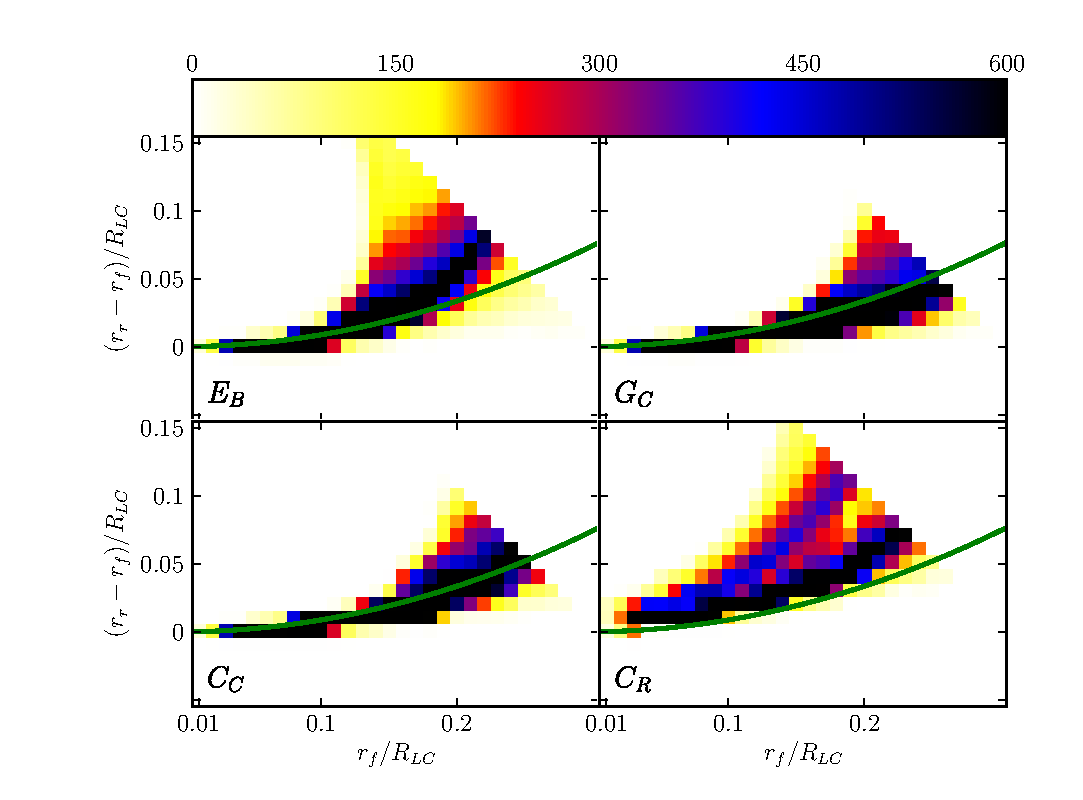
\includegraphics[width=.7\textwidth]{chapter2figures/totDirFitPhi.eps}
\special{psfile=chapters/radioDataAnalyticModels/figures/stokesFigure.eps hoffset=-100 voffset=-300 vscale=100 hscale=100}
\caption[Visualization of Stokes parameters]{
Visualization of Stokes parameters.  The absolute value of linear polarization ($|L|=\sqrt{U^2+Q^2}$ )
occupies the $U$-$Q$ plane while circular polarization $V$ is the third Cartesian axis.  The
total polarized intensity is labeled $pI$ and the total intensity which extends beyond
the polarized intensity is labeled $I$.
}
\label{fig:stokes}
\end{center}
\vskip -.03\textheight
\end{figure}

Stokes parameters are a convenient way of expressing polarization and is particularly useful for
describing partially polarized light using $p$. The Stokes parameters occupy the so-called
Poincar\'{e} sphere of optics where $Q$, $U$, and $V$ are the axes and $pI$ is the radius of the
sphere (Figure~\ref{fig:stokes}).  The polarization angle ($\psi$) and linear polarization ($L$) relate to the polar coordinates of
$Q$ and $U$:

\begin{equation}
    |L|=\sqrt{U^2+Q^2}
\end{equation}
\begin{center}
and
\end{center}
\begin{equation}
    \psi=\frac{1}{2} \arctan{\left(\frac{U}{Q}\right)}.
\end{equation}

Polarization data that we received from collaborators is in the form
of $Q$, $U$, $V$, $I$ versus pulsar rotation period phase and we
calculate polarization using $Q$ and $U$.

Further error bars for the polarization are calculated using the
following formula (standard error propagation):

\begin{equation}\sigma_{\psi}(\phi)=\frac{1}{2} \frac{\sqrt{\langle\sigma_{U{\rm off}}*Q(\phi)\rangle^2+\langle\sigma_{Q{\rm off}}*U(\phi)\rangle^2}}{\langle Q(\phi)\rangle^2+\langle U(\phi)\rangle^2}.\end{equation}

The values $\sigma_{Q{\rm off}}$ and $\sigma_{U{\rm off}}$ are the standard deviation in the off-pulse phases of $Q$ and $U$.
Note that $Q$, $U$, and $\sigma_{\psi}$ are all functions of the 
pulsar rotation period phase, $\phi$.

